\documentclass[conference]{IEEEtran}
%\IEEEoverridecommandlockouts
% The preceding line is only needed to identify funding in the first footnote. If that is unneeded, please comment it out.
\usepackage{cite}
%\usepackage[noadjust]{cite}
\usepackage{amsmath,amssymb,amsfonts}
\usepackage{algorithmic}
\usepackage{graphicx}
\usepackage{textcomp}
\usepackage{xcolor}
\usepackage{array,etoolbox,multirow}
\usepackage{float}
\usepackage{caption} 
\usepackage{multirow}
\captionsetup[table]{skip=6pt}

\def\BibTeX{{\rm B\kern-.05em{\sc i\kern-.025em b}\kern-.08em
    T\kern-.1667em\lower.7ex\hbox{E}\kern-.125emX}}
\begin{document}

\title{A domain-driven distributed reference
architecture for big data systems\\
}

\author{\IEEEauthorblockN{1\textsuperscript{st} Pouya Ataei}
\IEEEauthorblockA{\textit{School of Engineering, Computer and Mathematical Science} \\
\textit{Auckland University of Technology}\\
Auckland, New Zealand \\
pouya.ataei@aut.ac.nz}
\and
\IEEEauthorblockN{2\textsuperscript{nd} Alan Litchfield}
\IEEEauthorblockA{\textit{Service and Cloud Computing Research Lab} \\
\textit{Auckland University of Technology}\\
Auckland, New Zealand \\
alan.litchfield@aut.ac.nz}

}

\maketitle

% Rewritten parts to eliminate unnecessary verbiage, put preposition statements at the start of sentences and clarify language. Corrected spelling and grammar errors
 
\begin{abstract}
    The proliferation of digital devices, rapid development of software, and the availability of infrastructure augment the capability of users to generate data at an unprecedented rate. The accelerated growth of data has precipitated a shift in the industry which we perceive as the era of big data.  The era of big data began when the variety, velocity and volume of data overwhelmed traditional systems, and induced a paradigm shift in data engineering. While companies have attempted to harness the benefits of big data, success rates are still low. Due to challenges such as rapid technology change, organizational culture, complexities of data engineering, impediments to system development, and a lack of effective big data architectures, it has been estimated that only 20\% of companies have successfully institutionalized big data. By introducing a domain-driven distributed big data reference architecture, this study addresses issues in big data architecture, data engineering, and system development. The reference architecture is empirically grounded and evaluated through deployment in a real-world scenario as an instantiated prototype, solving a problem in practice. The results of the evaluation demonstrate utility and applicability with thought-provoking architectural tradeoffs and challenges.
\end{abstract}

\begin{IEEEkeywords}
Big data architecture, data architecture, big data, domain-driven distributed big data systems
\end{IEEEkeywords}

\section{Introduction}
% In this section: Rewritten parts to eliminate unnecessary verbiage, put preposition statements at the start of sentences and clarify language. Corrected spelling, punctuation, and grammar errors.
The ubiquity of digital devices and software applications allow users to generate data at an unprecedented rate. Almost all aspects of human life is integrated with some sort of software system that is performing computational processes on data. The rapid expansion and evolution of data from a structured
element that is passively stored in the database to something
that is used to support proactive decision making for business
competitive advantage, have dawned a new era, the era of
Big Data (BD). The BD era emerged when the velocity, variety, and volume of data overwhelmed existing system capability and capacity effectively and efficiently process and store data \cite{ataei2021neomycelia,AtaeiACIS}. 

BD is the practice of crunching large sets of heterogenous
data to discover patterns and insights for business competitive
advantage \cite{AtaeiHype}. Since the inception of the term, ideas have
ebbed and flowed along with the rapid advancements of
technology, and many strived to harness the power of BD. Nevertheless, there are many failed attempts, for example, as at 2021 only 13\%{} of organizations surveyed succeeded in delivering on their data strategy \cite{DataBricksSurvey} and 20--24\%{} successfully adopted BD \cite{NewVantageSurvey,GartnerSury}. Therefore, successful adoption of BD is scarce and apparent challenges include ``cultural challenges of becoming data-driven'', ``BD architecture'', ``data engineering complexities'', ``rapid technology change'', and ``lack of sufficiently skilled data engineers'' \cite{AtaeiBigDataEnvirons}.  

% Furthermore, 25\%{} of respondents in a survey of business experts experienced delays in data analysis and gave up searching for insights \cite{SigmaSurvey}. 



A big data system is motivated by an array of functional
requirements and quality goals. But if this system is to be successful, it must achieve these functional requirements within
an acceptable performance, availability, modifiability and cost
parameters. The software architecture is the key ingredient
in determining whether these goals are attainable, before
colossal amount of resources are committed to it. The initial
design, development and deployment of a BD system does
not mean success. As system grows larger, data providers and
data consumers increase, data variety expands, data velocity
extends, and metadata becomes increasingly more challenging
to handle. This means, only a handful of hyper-specialized data
engineers would be able to understand the system internals,
resulting in silos, burnt out and potential friction.

This creates a perfect ground for immature architectural
decisions that result in hard-to-main and hard-to-scale systems,
and raise high-entry blockage. Since ad-hoc BD designs are
undesirable and leaves many engineers and architects in the
dark, novel architectures that are specifically tailored for BD
are required. To contribute to this goal, we explore the notion
of reference architectures (RAs) and presented a domaindriven distributed software RA for BD systems.

%%%%%%%%%%%%%%%%%%%%%%
% In this section: 
%Rewritten parts to eliminate unnecessary verbiage
%Put preposition statements at the start of sentences
%Clarify language. 
%Corrected spelling, punctuation, and grammar errors. 
%Restructured the description lists. 
%Removed pejorative language. 
%Corrected acronym formatting.
%Added missing acronym definition
%Colloquial language formalised
%removed tautologies

\section{Background}
In this section, the current state of BD knowledge, identification of the study focus, and study objectives are provided. Two important elements are discussed, the current state of BD architectures and why RA is needed.

\subsection{Overview of BD architectures}
In this overview, three generations of BD architecture are presented. A key issue apparent in all these approaches is the underlying monolithic data pipeline architecture that channels all data without any consideration for data quality. Thus, data logically linked to specific domains are now lumped together and processed in one architectural quantum, creating impediments to scalability and maintainability.

\begin{LaTeXdescription}
    \item[Enterprise Data Warehouse] Generally built around a monolithic data warehouse, Extract-Transform-Load (ETL) processes, and data analysis and visualization/presentation software. Enterprise Data Warehouses are typically designed against specific requirements that limits how BD characteristics may be exploited effectively. As the Enterprise Data Warehouse expands and data consumers and data providers increase, then ETL processes become increasingly difficult to maintain and manage. This results in slower transaction processing and increased dependency on a small group of specialized staff. Such dependency creates silos that creates friction within and between teams and organizational boundaries. Furthermore, the monolithic architecture makes scaling, maintenance, and the extension of non-functional scope (for example, the addition of new transformations or data structures)  difficult and time consuming and thus, expensive.
    \item[Data Lake] to address some of the issues with data warehouses in general, a new BD ecosystem emerged as the Data Lake. In this approach, there isn't much data transformation before data are written into the Data Lake and retrieved when needed. While Data Lake architectures address some issues with data warehouse architectures, such as the capability of handling data variety, optimization features may be lacking. For example, if the number of data consumers and providers increase beyond the system's capacity to efficiently and effectively handle queries and manage data, then a data swamp may be created. Furthermore, data quality decreases over time firstly because no data owners are linked to stored data, and secondly because the BD stack is managed by specialized data engineers that may become siloed with ever-increasing backlogs. Data engineers may have little awareness of the semantics and value of the data they are processing, how data are useful to the business, and which domain data belongs to. Consequently, data quality reduces making maintenance and scaling a daunting task. 
    \item[Cloud Based Solutions] Considering the sheer cost of running a data engineering cluster on-premise, the current talent gap faced in the market, and complexity of provisioning the infrastructure of ever-increasing data processing loads \cite{AtaeiHype}, companies may choose to deploy on the Cloud for their BD solutions. The current technological generation leans towards architectures that provide Lambda or Kappa for stream processing or batch processing, or frameworks that unify the two like Databricks or Apache Beam. Whereas this generation of BD architectures might bring reduced cost and complexity for data architects, it still suffers from the same architectural challenges of having no clearly defined data domains, siloed specialized data engineers, and a monolithic pipeline BD architecture.
\end{LaTeXdescription}

To address these issues, we explore a domain-driven distributed RA for BD systems and propose an RA that addresses some of the challenges. The RA is inspired by the advances in software engineering architectures, and in specific microservices, domain-driven design, and reactive systems. 


\subsection{Why a Reference Architecture?}
Software architecture is an artefact that aims to satisfy business objectives through a software solution that is adaptable, cost-efficient, maintainable, and scalable. In addition, it allows for the capture of design issues at an early stage in the development process. Whereas this practice can be applied to any class of system, it is particularly useful in the design and development of complex system such as BD \cite{ataei2021neomycelia}. Despite the known complexity of BD systems, the development, analysis, and design of an RA incorporate best practices, techniques, and patterns that supports the achievement of BD undertakings is possible. Therefore engineers and architects can better absorb the complexity of BD system development and make it tractable. This approach to system development is not new for practitioners of complex systems. 

In Software Product Line (SPL) development, RAs provide generic artefacts that are instantiated and configured for specific system domains \cite{Derras}. Also, To address complex and unique system design challenges in software engineering, Information Technology (IT) giants like IBM refer to RAs as the `best of best practices'  \cite{Cloutier}. 


Furthermore, RAs are used to standardize an emerging domain, a good example of this is the \emph{BS ISO/IEC 18384-1 RA for service-oriented architectures} \cite{Iso18384-1} and in diverse environments like NASA space data systems \cite{NASA}.Therefore, RAs are effective for addressing complex BD system development, because: 1) RAs promote adherence to best practice, patterns, and standards, 2) RAs can endow the architecture team with increased openness and interoperability, incorporating architectural patterns that provide desirable quality attributes, 3) RAs serve as the locus of communication, bringing various stakeholders together. 

%%%%%%%%%%%%%%%%%%%%%%
% In this section: 
%Rewritten parts to eliminate unnecessary verbiage
%Put preposition statements at the start of sentences
%Clarify language. 
%corrected tense (present tense)
%Corrected spelling, punctuation, and grammar errors. 
%removed collective personal narrative statements
%Restructured the description lists. 
%Corrected acronym formatting.
%changed long form of terms to acronyms
%Colloquial language formalised
%removed tautologies
%fixed poorly structured citations
%added missing citations
%Corrected table cross-ref

\section{Research Methodology}
The study is comprised of two phases: the first is the identification of high level requirements of the artefact, and second applies a well-established methodology for building the RA. This section describes the process of the two phases and approaches were made.


\subsection{Requirement Specification}
Prior to RA modelling and design, the desired properties of the artefact are defined as requirements. System and software requirements range from a sketch on a napkin to formal (mathematical) specifications. Therefore, the kind of requirements for the purpose of this study are defined in an exploration of the body of evidence. An analysis of existing RAs developed for BD systems offers general requirements, the spectrum of BD RAs, and how they are designed \cite{ataei2020big}.  

Defining and classifying software and system requirements is a common subject of debate. Sommerville \cite{sommerville2011software} classify requirements as three levels of abstraction; user requirements, system requirements, and design specifications. These are mapped against user acceptance testing, integration testing, and unit testing. In this study, a more general framework provided by Laplante \cite{laplante2017requirements} is adopted. The adopted approach provides three categories as functional, non-functional, and domain requirements. The objective in this phase is to define the high-level requirements of BD systems, thus non-functional requirements are not fully explored. 

% For example, the majority of non-functional requirements emerge from peculiarities found in an environment like banking or healthcare, whereas this study focuses on a higher level. Therefore, the focus is on functional and domain requirements primarily, and then on non-functional requirements.

After clarifying the type of requirements, prior research provides general requirements for BD systems. The 5Vs of Velocity, Veracity, Volume, Variety and Value are frequently referenced \cite{Bahrami2015,rad2017big,Chen2016a}. In an extensive effort, NIST Big Data Public Working Group embarked on a large scale study to extract requirements from variety of application domains such as Healthcare, Life Sciences, Commercial, Energy, Government, and Defense \cite{Chang}. The result of this study was the formation of general requirements under seven categories. Volk et al. \cite{volk2020identifying} categorizes nine use cases of BD projects sourced from published literature with a hierarchical clustering algorithm. Bashari et al. \cite{bashari2016security} focus on security and privacy requirements for BD systems, Yu et al. present modern components of BD systems \cite{yu2019components}, using goal oriented approaches, Eridaputra et al. \cite{eridaputra2014modeling} create a generic model for BD requirements, and Al-jaroodi et al. \cite{al2016characteristics} investigate general requirements to support BD software development. 



By analyzing these studies and by evaluating the design and requirement engineering required for BD RAs, a set of high-level requirements based on BD characteristics is established. A rigorous approach to present software and system requirements that offers informal methods of model verification is identified because such methods are well established in the industry and academia \cite{kassab2014state}.  The approach for representing functional requirements follows the guidelines in \emph{ISO/IEC/IEEE standard 29148} \cite{ISO29148}. The requirements representation is organized in system modes, where the major components of the system and then the requirements are described. This approach is inspired by the requirement specification expressed for NASA Wide-field InfraRed Explorer (WIRE) system \cite{laplante2017requirements} and the Software Engineering Body of Knowledge (SEBoK) \cite{abran2004software}.

The requirements are categorized by the major characteristics of BD (Table~\ref{table-requirements}); value, variety, velocity, veracity, volume \cite{rada2017hype}, and security and privacy \cite{bashari2016security}. 

%\begin{center}
    \begin{table*}[h]
    \centering
    \renewcommand*{\arraystretch}{1.8}
    \begin{tabular}{|m{1.2cm}|m{16cm}|}

        \hline

        Volume &

        \textbf{Vol-1)} System needs to support asynchronous, streaming, and batch processing to collect data from centralized, distributed, and other sources, \textbf{Vol-2)} System needs to provide a scalable storage for massive data sets 
        \\
        \hline
        Velocity & 
        
        \textbf{Vel-1)} System needs to support slow, bursty, and high-throughput data transmission between data sources, \textbf{Vel-2)} System needs to stream data to data consumers in a timely manner, \textbf{Vel-3)} System needs to be able to ingest multiple, continuous, time varying data streams, \textbf{Vel-4)} System shall support fast search from streaming and processed data with high accuracy and relevancy, \textbf{Vel-5)} System should be able to process data in real-time or near real-time manner 
        \\ 

        \hline

        Variety & 

        \textbf{Var-1)} System needs to support data in various formats ranging from structured to semi-structured and unstructured data, \textbf{Var-2)} System needs to support aggregation, standardization, and normalization of data from disparate sources, \textbf{Var-3)} System shall support adaptations mechanisms for schema evolution, \textbf{Var-4)} System can provide mechanisms to automatically include new data sources 
        \\

        \hline

        Value & 
        
        \textbf{Val-1)} System needs to able to handle compute-intensive analytical processing and machine learning techniques, \textbf{Val-2)} System needs to support two types of analytical processing: batch and streaming, \textbf{Val-3)} System needs to support different output file formats for different purposes, \textbf{Val-4)} System needs to support streaming results to the consumers 
        \\

        \hline

        Security \& Privacy & 
        
        \textbf{SaP-1)} System needs to protect and retain privacy and security of sensitive data, \textbf{SaP-2)} System needs to have access control, and multi-level, policy-driven authentication on protected data and processing nodes. 
        \\

        \hline
        
        Veracity &
        
        \textbf{Ver-1)} System needs to support data quality curation including classification, pre-processing, format, reduction, and  transformation, \textbf{Ver-2)} System needs to support data provenance including data life cycle management and long-term preservation.
        \\
        \hline
  
    \end{tabular}
    \caption{BD system requirements}
    \label{table-requirements}
    \end{table*}
%\end{center}


\subsection{Artefact Development Methodology}
There are several approaches to the systematic development of RAs. Cloutier et al \cite{Cloutier} demonstrate a high-level model for the development of RAs through the collection of contemporary architectural patterns and advancements. Bayer et al \cite{bayer1999pulse} introduce a method for the creation of RAs for product line development called PuLSE DSSA. Stricker et al \cite{stricker2010creating} present the idea of pattern-based RA for service-based systems and use patterns as first class citizens. Similarly, Nakagaw et al \cite{nakagawa2014consolidating} present a four-step approach to the design and development of RAs. Influenced by ISO/IEC 26550 \cite{wg2015iso}, Derras et al \cite{Derras} present a four-phase approach for practical RA development in the context of domain engineering and SPL.

% Nguyen et al \cite{nguyen2010methodology} utilize reverse engineering and a reference model for the creation of an agent-based systems RA, and Norta \cite{norta2006developing} follow a pattern-based approach similar to that of Stricker et al \cite{stricker2010creating}. 



% Analysis and study of these methodologies for the design and development of RAs highlight several recurring themes: RAs should capture the essence of best practice; RAs can be built by absorbing current best practice, standards, architectures, RAs, and systems; and RAs should sit at the right level of abstraction.

Additionally, Galster \cite{GALSTER} and Avgeriou \cite{Avgeriou} propose a 6-step methodology with two primary concepts: empirical foundation and empirical validity. Taking all these into consideration, an empirically-grounded RA methodology proposed by Galster and Avgeriou provides the most appropriate methodology to meet the purposes of this study. Reasons being that this methodology for RA development is adopted more than any other, and that the methodology supports the objectives of this study. 

Nevertheless, this methodology suffered from a few limitations and we had to augment several areas of it with
other approaches in order to arrive at the desired rigour and
relevance.  For instance, we could not find comprehensive
guidelines on how to collect empirical data in step 3 of
the methodology. We did not know what kind of theory we
should collect and how should we model the data collected.
Thereby, we employed Nakagawa et al’s information source
investigation guidelines and the idea of RAModel [39].

Also, the methodology does not describe how to evaluate the RA, thus, a more systematic and stronger evaluation approach is required. To address this, an instantiation the RA is deployed in a real world practice, then the Architecture Tradeoff Analysis Method (ATAM) \cite{KazmanATAM} is applied to evaluate the artefact. The methodology constitutes 6 steps: 1) Decision on type of the RA, 2) Design strategy, 3) Empirical acquisition of data, 4) Construction of the RA, 5) Enable RA with variability, 6) Evaluation of the RA. 



\begin{LaTeXdescription}
\item[1. Decision on type of the RA] Prior to the development of the RA, the type needs to be identified. The type determines the structure, the data to be collected, and the objective of the RA. To determine the type of RA, a classification framework provided by Angelov et al \cite{angelov2009classification} is applied and a Systematic Literature Review (SLR) \cite{AtaeiACIS}. 

In this classification framework, RAs are categorized as standardization RAs and facilitation RAs. The domain-driven distributed RA chosen for the purposes of this study addresses two essential goals: 1) openness and interoperability between heterogenous components of a BD ecosystem and 2) facilitation of BD system development and data engineering. Accordingly, the output artefact is classified as `classical standardization RA designed to be implemented in multiple organizations'. 

%%%%%%%%%%%%%%%%%%%%%%%%%%
%%%%%.  I got this far %%%%%%%%%%%%%%
%%%%%%%%%%%%%%%%%%%%%%%%%%


\item[2. Selection of Design Strategy] According to Galster et al \cite{GALSTER}, RAs can have two major design strategies to them; 1) RAs that are based on existing patterns, principles and architectures, and 2) RAs that are developed from scratch. Designing RAs from scratch is scarce and usually happens in areas that have received no attention (could be BD in 2004). On the other hand, RAs are proven more successful when built from the proven practices \cite{Cloutier}. 

The RA developed for the purposes of this study is a research-based RA based on existing RAs, concrete architectures, patterns, standards and best practices.

\item[3. Empirical Acquisition of Data] Due to limitations witnessed by the Galster et al's methodology, we have augmented this phase to increase transparency and systematicity, by employing a SLR for data collection. 

This phase is comprising of three major undertakings; 1) identification of data sources, 2) capturing data from the selected sources and 3) synthesis of the selected data. 

\emph{Identification of Data Sources:} For this sub-phase, we employed the ProSA-RA's 'information sources investigation'. To unearth the essential architectural quanta, we selected our sources as 'publications'. In order to capture the essence of existing body of knowledge from publications, we conducted a SLR. This SLR is an extension of Ataei et al work \cite{AtaeiACIS} which covered all the RAs by 2020. We followed the exact methodology as described in \cite{AtaeiACIS}, but this time for the years 2021 and 2022. The main objective of this SLR is to find common architectural constructs among existing BD architectures, and highlight limitations.



\emph{Capturing data from the selected sources:} After having pooled quality literature, the study embarked in the process of capturing data. We used to software Nvivo for coding, labelling and classifying studies. 

\emph{Synthesizing Data:} Codes highlighted patterns and patterns resulted in themes, which grounded the design theories necessary to build this RA. Our aim was to capture the body of knowledge and project it into our RA. 

% The themes emerged from this SLR and the literature review we've done for requirements specification sometimes overlapped. The focus of this SLR was primarily on capturing architectural constructs defined in the conceptual framework of the studies, while the focus of the literature review conducted for requirement specification was regarding only the system and software requirements. It was necessary to first understand what needs to be built, and then search for actual artefacts.

\item[4. Construction of the RA] Based on the requirements, themes, patterns and theories emerged from the previous step, the design and development of the RA initiated. Integral to this phase is the components that the RA should contain, how they should be integrated, how they should communicate, how do they address the requirements and what are the architectural tradeoffs. 

To describe the RA, we followed ISO/IEC/IEEE 42010 standard \cite{ISO42010}. As suggested by the standard, we used Archimate to model our architecture.

% This standards is tailored for concrete architectures, so we did not fully conform to it, but rather the good and relevant parts are taken. 

% For instance, expression of the architecture through architectural description language (ADLs), architecture viewpoints, and statements of corresponding rules have had great influence in the design adn development of this RA. 

% A key challenge was perhaps determination of right level of abstraction; to strike a balance between the specificity of micro-patterns and generality of high-level architectural approaches. 

% In our observation, BD RAs today to do not adhere to a common vocabulary for architectural descriptions, and most RA developments are driven by a small set of lexicon that author defines and utilizes for representation. This makes the process of analysis and comparison more difficult, as there is no level playing field. 

% We've been faced two major challenges: 1) determining the right level of abstraction, and 2) delineation of the RA. In our observation, BD RAs todays do not adhere to a common vocabulary for architectural descriptions, and most RA developments are driven by a small set of lexicon that author defines and utilizes for representation. This makes the process of analysis and comparison more difficult, as there is no level playing field. 

% Inspired by the body of evidence, and illuminated by the limitations we've witnessed in other studies, we decided to adhere several architectural views into on and express it through a multi-layer modelling language called Archimate. 

% Archimate has been chosen firstly because it is a mature language developed by the collaboration of academics and practitioners through the umbrella of Open Group, and secondly because it is listed as a standard Architecture Description Language (ADL) in ISO/IEC/IEEE 42010. 

\item[5. Enabling RA with variability] One of integral elements that help with instantiation of the RA is variability. This enables RA to remain useful as a priori artefact when it comes down to organization-specific regulations, and regional policies that may constrain the architect's freedom in design decisions. For the purposes of this study, we chose to represent variability by the means of ``annotation'' as recommended as on of the three accepted approaches by Galster et al \cite{GALSTER}.

% Clear identification of RA do also facilitate communications among stakeholders and affect artefact evaluation and tradeoff analysis. 

% Variability management is a well studied concept in Business Process Management (BPM) \cite{la2009questionnaire}, and Software Product Line Engineering (SPLE) \cite{pohl2005software}. 



% and whereas BPM focuses of efficient handling of variables in business processes, SPLE tends to focus on handling variants in software artefact to account for emerging requirements. 

\item[6. Evaluation of the RA] This last phase of the methodology is to ensure that RA has achieved its goal, and to test its effectiveness and usability. Based on Galster et al's \cite{GALSTER} work, a quality of the RA can be deduced based on its utility, correctness and how efficiently it can be adopted and instantiated. Howbeit, the evaluation of the RAs is a known challenge among researchers \cite{Avgeriou}, and while there are many well-established methods for assessing concrete architectures, many of these methodologies fall short in evaluating RAs. 

This is due to the inherent properties of RAs such as level of abstraction, and lack of clearly defined group of stakeholders. Various authors have attempted to solve this issue; for instance, Angelov et al's \cite{angelov2008towards} attempt on modifying ATAM and extended it to resonate well with RAs. To this end, we first instantiated the RA, and then evaluate the prototype in practice, using ATAM. 


% Taking all the factors into consideration, and to provide with a rigorous evaluation,


\end{LaTeXdescription}


\section{The Artefact}

% If the aspiration to enhance every business aspect with data needs to come to fruition, there is a need for a different approach to BD architecture. Traditional approaches to data storage and crunching, while proven to be effective in handling volume aspect of data, fall short in addressing other characteristics of it; increased heterogeneity and proliferation of data sources (variety), the rate at which data arrives and needs to be processed (velocity), the quality and provenance of data (veracity), and the rate at which data mutates (variability).


% \subsection{A Domain-driven Distributed RA for BD Systems}

The RA is built underlying several principles: 1) Domain-driven: to address data quality, siloed teams, data swamp issues and communication issues, affecting velocity, variety, and veracity requirements; 2) Distributed: to address the challenges of scaling monolithic data systems affecting velocity, and volume requirements; 3) Data as a service: to allow for increased discoverability of data and autonomy of various analysis and data science teams without frictions with data engineers affecting value, variety, veracity, security and privacy requirements; 4) Governance through a federated service: the prevent team-based and rather immature decisions that may not be in-line with global organizational visions, policies, standards and procedures, affecting all requirements; 5) Event driven: to address point-to-point communication issues that arises in distributed systems, affecting velocity requirement. 

Lastly, it is worth mentioning that many of our designs have had inspirations from microservices architectural patterns \cite{richardson2018microservices}. Based on these principles, the RA designed for the purposes of this study is presented in \ref{fig-RA}. We have chosen this artefact to be domain-driven and distributed in order to shift from collecting data in monolithic data lakes and data warehouses to converging data through a decentalized and distributed mesh of data products communicating through standard interfaces. This is directly addressing the limitations discussed with current BD architectures. 

This RA is made up of 11 main components and 9 variable components, these components are briefly discussed as below:

\begin{figure*}[h]
    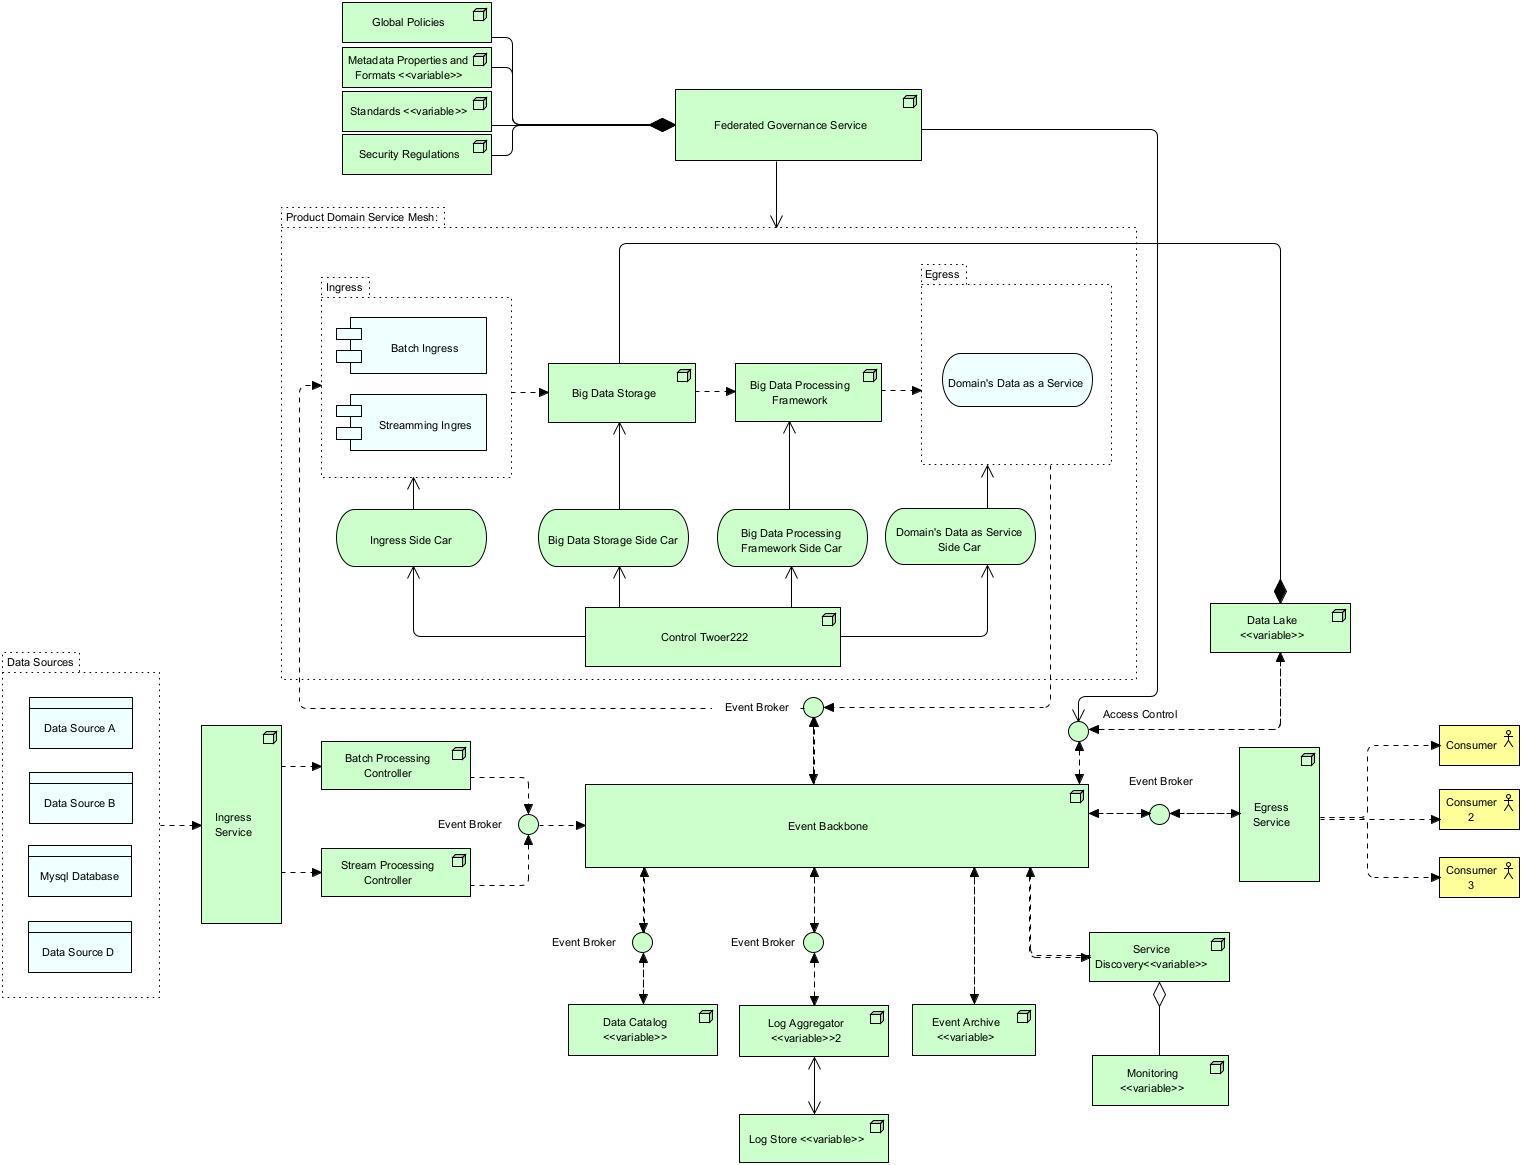
\includegraphics[width=17cm]{media/Metamycelium.jpg}
    \caption{domain-driven Distributed RA}
    \label{fig-RA}
\end{figure*}


\begin{enumerate}
    \item \textbf{Ingress Service:} this service is responsible for controlling traffic into the system. Depending on the nature of the request, this service will load balance either into a batch processing controller or a stream processing controller. Ingress is an asynchronous load balancer designed to eliminate choke points, handle SSL termination, and provide with extra features such as named-based virtual hosting. This component addresses the requirements Vol-1, Vol-2, Var-1, Var-3, Var-4, Val-1, Val-3, Val-4, SaP-1 and SaP-2. 
    
    % Having defined ingress allows for clear demarcation of the system boundaries, eliminates performance affecting security measures to be taken care of, allows for more private networks within the system, and can be used to augments objects too. 

    \item \textbf{Batch Processing Controller:} this controller is responsible for handling batch processes. That is, it is responsible for receiving request for batch processing, and communicating it to the event broker. Due to the batch nature of the requests, the controller can decide to achieve this in a bulk and asynchronous manner. This component addresses the requirements Vel-1, Val-1, and Val-2. 
    
    % This controller as opposed to its stream processing counterpart, can execute non compute-intensive proxy operations if needs be.
    \item \textbf{Stream Processing Controller:} This controller achieves similar thing to the batch one, with a difference that it has to handle a different nature of requests. Stream events are synchronous in nature and require hight through-put. Having a specific service for stream processing requirements promote tailored customization that best suit the varying nature of stream events. This component addresses the requirements Vol-1, Vel-1, Vel-2, Vel-4, Vel-5, Val-2,  
    
    \item \textbf{Event Broker:} event broker is an important architectural construct designed to achieve 'inversion of control'. As the system grows, more nodes and services are added, communication channels increase, and there is a need fore new events to be dispatched. As each service communicates through the event backbone, each service will be required to implement its own event handling module. This can easily turn into a spaghetti of incompatible implementations by different teams, and can even result in unexpected behaviors. To address this issue, an event broker is introduced to each service which has one main responsibility; communication with event backbone. This component indirectly addresses the requirements Val-1, and Ver-1.  
    
    % This means services are no longer required to implement their own event handling functions, and this responsibility is given to the event broker instead. One of the key success criteria for event brokers is a unified interface that resides in a right level of abstraction to account for all services of the architecture.
    \item \textbf{Event Backbone:} Event backbone is the heartbeat of the system, facilitating communication between all services. Where as this service is displayed as one technology service in the Archimate diagram, we recommend the event backbone to be designed underlying distributed paradigms itself. This is to ensure scalability as the number of topics and events grows. Event backbone and its relations to other nodes is analogous to a dance troupe; in a dance troupe, the members respond to the rhythm of music by moving according to their specific roles; the same happens here, with a difference that this time, event backbone is the music and services are the members of the dance troupe. This implies that services are only responsible for dispatching events in a 'dispatch and forget' model, subscribing to topics they are interested. This component addresses the requirements Vel-1, Vel-2, Vel-3, Vel-4, Vel-5, Val-1, Val-2, Ver-1, Ver-2, and Ver-3.
    
    % Whereas networking challenges remain the same, this approach solves myriad of challenges associated with point-to-point communication.
    \item \textbf{Egress Service:} This services is responsible for providing necessary APIs to the consumers of the system, third parties or other BD systems. This allows for the openness of the architecture, and lets data scientist and business analyst easily request the data necessary for their work-loads. This also promotes the idea of self-serve-data through service discovery, data catalogue and product domains. This component can also be tuned for QoS networking, and other low computational functions if needs be. This component addresses the requirements Vel-2, Vel-4, Val-3, Val-4, SaP-1, and SaP-2. 
    
    % Systems or scientists can first request for a data catalogue and then use the catalogue to request for the required data. The egress services handles the traffic necessary for these requests to be successful. This component can also be tuned for QoS networking, and other low computational functions if needs be. 
    \item \textbf{Product Domain Service Mesh:} Driven by the idea of domain-driven design, every product has it is own bounded context and ubiquitous language, and is technically governed by a service mesh. Every service mesh is made up of a batch ingress, stream ingress, BD storage, BD processing framework, domain's data service, together with the control tower and the side cars. These components provides the necessary means for the domain to achieve its ends in regards to BD processing. This is to enable high cohesiveness, low coupling and clear interfaces among services. This component indirectly addresses Vol-1, Vel-3, Vel-4, Vel-5, Var-1, Var-2, Var-3, Val-1, Val-2, Val-3, Val-4, Sap-1, SaP-2, Ver-1, Ver-2, and Ver-3.
    
    \item \textbf{Federated Governance Service:} Given the distributed nature of the architecture and sheer number of moving parts with varying life-cycles; there is a need for some global contextual standards and policies that are designed to streamline processes and avoid losses. This is not to limit the autonomy of teams, but to inject them with best practices and organizational policies that tend to reflect the capability framework, regional limitations, and legal matters that can cause sever damage to the business. This component can indirectly affect all requirements.
    
    % For instance, not every data engineer may be fully aware of various aspects of GDPR, or different teams may choose to embark on different event deduplication processes; for the former, one can adopt a global privacy policy rule, and for the latter, one can pick up Async API specifications. 
    \item \textbf{Data catalog:} As data products increase in the system, more data become available, interoperability increases, and thus services have to know who provides what data. Data catalog is responsible for keeping a catalog of all data available among services with relative paths to fetch those data. This component addresses the requirements Vel-4, Var-1, Var-3, and Var-4.

    \item \textbf{Log Aggregator and Log Store:} Operating underlying a distributed paradigms, requires a shift in a way that logging occurs. This means system cannot rely only one applications reporting logs in a single environment, but there's a need for a distributed tracing that shows a lifecycle of a process and how it went through different services. Therefore this RA benefits from the popular log aggregator pattern initially released by the microservices community, to allow fo graceful scaling of system's logging strategy. This component indirectly addresses the requirements Vol-1, Vel-1, Val-1, and Ver-1. 
    
    \item \textbf{Event Archive:} One of the main challenges of this architecture is it is reliance on event backbone. Whereas event backbone itself is recommended to be distributed and fault tolerant, event archive further solidifies the service recovery from unexpected events. This implies that, if the event backbone went out of service, the history of events can be stored and retrieved from the event archive to bring various services to the current state of operation. This component indirectly addresses the requirements Vol-1, Vel-1, Val-1, and Ver-1. 

    \item \textbf{Data Lake:} Whereas product domains are demarcated and boundaries are well-defined, we do not find it necessary for each domain to maintain it is own data lake. This is under the assumption that a lot of data are now processed at the time of storage, and is required whenever there is a analytical business case for it. Whereas there isn't a data lake per domain, different domains can have a quota in the data lake that is owned and handled by access control. This component addresses the requirements Vol-2, Vel-1, Var-1, Var-3, Var-4, Val-3.
    
    \item \textbf{Service Discovery:} In a distributed setup like the one portrayed, services need to find each other in order to communicate their means. 
    
    % A naive way to achieve this could be the storage of service addresses in configuration files in services interested to know about a particular service. This soon becomes out of hand, is hard to scale and hard to maintain. 
    
     Service discovery solves this issue with primary responsibility of identifying services and answering queries about services. This is achieved by services registering themselves to service discovery on boot up. This component indirectly addresses the requirements Vel-2, Vel-4, Var-2, Var-4, Val-3, Val-4, SaP-2. 

    \item \textbf{Monitoring:} Last, but not least, in order to take proactive measures for the overall health of the system and its considerable moving parts, one needs to actively monitor the state of the individual nodes and the overall flow of things. Services emit large amounts of multi dimensional telemetry data that can be read and analyzed for the supporting actions. Monitoring services help storing these data to fuel proactive actions. This component indirectly addresses all requirements. 

\end{enumerate}

The elements of the RA that are annotated with the phrase 'variable' can be modified, adjusted or even omitted based on the architect's decision. 

% It is als worth mentioning that what's provided is a brief explanation of these elements, and each element's description can be extended to a considerable amount. 

% The aim of this RA is not limit the creative of software architects, but to facilitate their decision making process. 

\section*{Evaluation}

Of utmost importance to development of the RA, is the evaluation of it. Our aim is to evaluate the correctness and utility of the RA by how it can turn into a context-specific concrete architecture that solves an actual problem. For this purpose ATAM has been chosen. ATAM has been chosen because it's got a good pedigree both in academia and industry, and has been applied to variety of architectures in different scales \cite{SoftwareArchitectureKazman}. 

Using ATAM increased our confidence by uncovering key architectural tradeoffs, risks, and sensitivity points. While ATAM is usually conducted by an outside team after the architecture is created, we tailored it to the requirements of our study. We first created a prototype of our reference architecture, and then followed the ATAM steps to evaluate our prototype in a real-world setup. This approach helped us understand the consequences of our architectural decisions in a rigorous manner.

It is important to note that, this wasn't a setup in which an outside evaluation team would come to a company to evaluate an architecture in practice, but it was our prototype that we brought into a company to test its utility and relevance. While we could have achieved this with technical action research, we found ATAM to be in-line with our conceptual constructs, which is an architectural construct, that is ATAM provided us with a framework to discuss architectural concepts in a rigorous way \cite{wieringa2014design}. 

For instantiation fo the RA, We utilized ISO/IEC 25000 SQuaRE standard (Software Product Quality Requirements and Evaluation) \cite{ISO25000} for technology selection. 

% We found mature technologies that could support our requirements, and opted not to develop any tools from scratch for the purposes of this study. It is also worth mentioning that, 

We chose Node JS for all APIs and custom scripting, Nginx as our ingress, AWS Lambdas for stream and batch processing controllers, Kafka for event backbone, Kafka event brokers as the event broker, AWS application load balancer as the egress load balancer, Istio as the control tower, Envoy as the side car, Kubernetes as the container orchestrator, AWS S3 as the BD store and event archive, and Data Bricks for stream and batch processing. 


We aimed to incorporate most components of our RA into this instance, however logging, monitoring, service discovery, federated governance service, and data catalog has been omitted. For brevity purposes, we dot not expand on ATAM steps in detail or the benefits of it, and we only explain how the evaluation has been conducted. Some details of this evaluation is omitted to protect the security, and intellectual property of the practice, and some details are modified for academic purposes. These modifications have not affected the integrity of the evaluation.  

\subsection{Phase 1:}

Evaluation has taken place in a subsidiary of an international large-scale company. The subsidiary company is specialized in practice management software for veterinary professionals visa Software as a Service ( SaaS ) providing services to hospitals all around the globe, among which is some of the biggest equine hospitals, and universities. The company has several ambitions, one of which is big data an AI. 

Following the guidelines of ATAM, the first step was the identification of relevant stakeholders. Our emphasis was on key stakeholders such as lead architects. This was important to ensure that we have not missed anything major in our design. We also opted not to include stakeholders that do not directly correlate with the prototype, such as the UI/UX designer. As a result, we invited two lead development architects, head of product, a product owner responsible for the product in which the artifact is tested, a quality assurance engineer and several developers. 

\subsubsection{Introductory Presentations}

During the initial meeting, in step 1, ATAM was presented with clear description of its purposes. In step 2, stakeholders discussed the background of the business and some of the challenges faced, and the current state of affairs, the primary business goals, and architecturally significant requirements. In step 3, From there on, the prototype has been presented, our assumptions have been stated, and variability points portrayed. 

\subsubsection{Identifying Architectural Approaches}


% We classified our architecture as micro-services. This was easier to grasp than 'domain-driven distributed architecture' for the stakeholders.

In this step, we discussed architectural styles in regards to quality attributes. For availability, we discussed Kafka's partitions, Nginx worker connections, Data Lake and Istio.  For performance, we discussed Nginx asynchronous processing, Kafka topics and consumers, AWS application load balancer, and Kubernetes deployments. For modifiability, we discussed the concept of domain-driven design, side cars, and event brokers. We then continued to analyze these approaches for tradeoffs, sensitivity points, and potential risks. 


\subsubsection{Utility Tree Elicitation}

In order to generate the utility tree, we first needed consensus on the most important quality attributes for this evaluation. We presented our assumptions and after a discussion, despite the fact that there were some concerns over privacy, the members agreed on availability, performance, and maintainability as the most important quality attributes. Based on that, we created the utility tree with the requirements of; 1) performance: system should be able to process real time streams under 1200 ms, queries from data scientist should not take more than 2 hours 2) availability: load balancer and data bricks cluster being available 99.999\% of the time, and 3) modifiability: new product domain should be added with less than 5 person in a month time.

We skipped the preliminary analysis of architectural approaches in phase 1 due to resources constraint, and only conducted it after the scenarios have been prioritized. This has not affected our overall evaluation process negatively.



\subsection{Phase 2:}

% After the selection of appropriate scenarios and several good cases for BD processing, we instantiated the RA. We utilized ISO/IEC 25000 SQuaRE standard (Software Product Quality Requirements
% and Evaluation) \cite{ISO25000} for technology selection. This prototype is a partial instantiation of the RA, that is aimed to solve a context specific problem. 

% We found mature technologies that could support our requirements, and opted not to develop any tools from scratch for the purposes of this study. It is also worth mentioning that, 

% As for the technology choices, we chose Node JS for all APIs and custom scripting, Nginx as our ingress, AWS Lambdas for stream and batch processing controllers, Kafka for event backbone, Kafka event brokers as the event broker, AWS application load balancer as the egress load balancer, Istio as the control tower, Envoy as the side car, Kubernetes as the container orchestrator, AWS S3 as the BD store and event archive, and Data Bricks for stream and batch processing. 

% (we used company's already in production data lake, with a test bucket in a staging environment)




\subsubsection{Scenario Prioritisation}

Scenarios are the quanta of ATAM, and help capturing stimuli to which the architecture has to respond. Based on this premise, in this step, we asked stakeholders to priorities three class of scenarios namely 1) growth scenarios, 2) use-case scenarios and 3) exploratory scenarios. As a result of this we pooled 20 scenarios, which we then asked stakeholders to vote on. The voting process yielded 5 scenarios, described as two user journeys; 1) The pet owner brings the pet to the veterinary hospital, the pet is diagnosed with cancer. The pet's environmental factors should be studied for potential clues on the root cause of cancer; 2) A pet owner brings the pet to the veterinary hospital, the cat symptoms should be processed for early detection of lyme disease. 



\subsubsection{Analyze Architectural Approaches}

After identifying architectural approaches and prioritizing scenarios, we ran the scenarios against our prototype. This is to provide heuristic qualitative analysis and point out sensitivity points and tradeoffs. We initiated this process by creating a custom script that extracts actual data from the company's mySQL database, and send it through the ingress. We created the necessary topics for Kafka, and configured Nginx to pass the requests to responsible lambdas for batch and stream processing. We then followed with event producers, Istio, Envoy, Kubernets, Data Bricks and the rest of the system. We then explained how our architectural decisions contribute to realizing each scenario.

\subsection{Present the Results}

In the process of running the scenario simulations against our system, we constantly probed our architectural approaches. 
Many implementation details arose in the process, and many sensitivity points annotated. We realized the true cost of the system, its trade offs and potential challenges. Based on these premises, and stakeholder feedbacks, we deduced that system quality Q\textsubscript{S}, is a function f of the quality attributes performance Q\textsubscript{P}, availability Q\textsubscript{A}, and modifiability Q\textsubscript{M}, as the equation Q\textsubscript{S} = fQ(Q\textsubscript{P}, Q\textsubscript{A}, Q\textsubscript{M}).

For performance, we used the cloud stress testing agent called StressStimulus. We ran the stress test against our system a couple of times, which revealed some interesting insights. It became evident that cold start time (100-1000ms) of AWS Lambdas can affect the desired performance. On the other hand, using Data Bricks for stream processing, we opted not to use micro-batch to have an accurate evaluation, we also decided not to configure the fair scheduling pool, so as to test the worst case scenario. 

% One solution to this was replacement of Lambdas with EC2 instance, but we opted not to do that, because this would affect maintainability negatively, as each EC2 instance needs provisioning and maintenance. 

After analyzing the prototype with various performance models (periodic data dispatch, large volume of data, many concurrent requests), it became evident to us that latency, input/output, and object mutations were the performance sensitivity points. The event driven nature of the system really shined at handling various simulations. Based on these findings, we characterize system's performance as  Q\textsubscript{P} = h(l, s, c). That is, system is sensitive to latency (l), side effects (s), and concurrency (c).

Next, we tested our prototype from availability point of view. Since the system is distributed in nature, the failure in one service, if not handled properly, can have a ripple effect on all services. Our prototype could easily recover from such situation through implementation of circuit breakers in event brokers. Our prototype also archived the events before the failure occurred in the event backbone, to bring back the system to a correct state. Moreover, we set up health checks and alarms on pods in the Kubernetes cluster and constantly monitored for system behaviors. 

% Another area were we initially worried a lot about, was the event backbone and fear of it turning into ESB of SOA, but that was certainly not the case, given that we designed the RA with the idea of a distributed backbone in it self. 


Kubernetes made sure that certain amount of services are always available through special services called deployments and replica sets. This evaluation has also made us realize that our architecture is compliant with twelve factor methodology and can be deemed cloud native. This has positively affected the availability score. Given all, we characterize the system's availability as $Q\textsubscript{A} = g(\mu\textsubscript{C}, \lambda\textsubscript{E}, \mu\textsubscript{S})$. That is, system availability is affected by the time it takes for circuit breakers to trip and become available again ($\mu\textsubscript{C}$), failure of the event backbone ($\lambda\textsubscript{E}$), and the time it takes for the services to recover ($\mu\textsubscript{S}$), with g being fraction of time that system is operating.

Lastly, we tested our prototype from modifiability point of view. The distributed and domain-driven nature of our architecture allowed us to easily achieve the desired modifiability objectives and even beyond. Adding a new data domain only required us to extend our HCL module written in Terraform for our EKS cluster, and modify it with new Docker images. Brokers were also streamlined, so we could spin up a new broker within minutes. We did not have to worry about certification lifecycle as it was handled by Istio, Local Cert Manager and Let's Encrypt. 

% Areas that we found more challenging was a bit more vendor specific. For instance, Databricks cluster optimisation, configuring Nginx as EKS ALB ingress, and handling ECR secrets and having them stored as Kubernetes secrets was not straight forward. 

Taking all into consideration, we characterize system's modifiability as $ Q\textsubscript{M} = s(K, K, D)$. That is, system modifiability is sensitive to Kafka provisioning, maintenance and configuration, Kubernetes maintenance, provisioning and configuration, and Databricks provisioning, configuration and maintenance, with s being the skill set required. 

\subsubsection{Tradeoff Points:}

After clear analysis, two tradeoff points have been identified; 1) event brokers and the event backbone and 2) service mesh. One area that raised concerns was the event backbone, and how it might turn into a bloated architectural component analogous to ESBs in SOAs. However, given the distributed nature of the system, event archive, and event brokers, we do not find that likely to happen. This architectural component is designed itself underlying the distributed principles and is responsible only for one function; communication among services. In addition, in the case of service outage, event archive can be utilized to retrieve the order of events, which in turn brings system to the correct state. Event brokers on the other hand, facilitate modifiability by providing native event handling mechanisms, but at a cost of one more layer and potential latency that comes with it. Given these, we deduced that event backbone while affecting performance and maintainability positively, can potentially have negative impact on availability and reliability. 
 
% During the tradeoff discussions, many other quality attributes have been discussed that are omitted for the purposes of this study. 
On the other hand, we realized, event brokers have positive effect on modifiability and availability, without having much negative effect on performance. One other area that was discussed heavily was the service mesh. Many developers found a lot to be done before the service mesh can operate and be up and running. We argued that while the initial effort for bringing up a service mesh may sound daunting, modifiability is positively affected longitudinally. Service mesh also promoted the concept of clear interfaces, separation of concerns, and a well-defined bounded context. Based on that, we deduced that service mesh has affected modifiability positively, but it might affect performance negatively due to the network communications required among services. 

% It also freed many developers from platform work that they usually don't excel at. 

%  Given all, even though we designed our RA with event back bone or a service mesh, we do not strongly prescribe these pattern. Our aim is not kill to creativity of software architects, but to shed lights on new ways of doing things with battle proven patterns. 
 
 Two limitations discussed among stakeholders was 1) complexity of implementing the design and 2) tail latency. For the former, we do not think that a distributed big data architecture should be simple; we simply do not recommend organizations to embark on this journey if they do not have the resources necessary to absorb the complexity. For the latter, we do not have a straight forward solution. This is a well known issue in the microservices community as well, and is addressed in our design by the means of fault-tolerant services.  


 

\section{Related Work}

Application of RAs to solving some of the challenges of data architecture is not a new concept. In one instance, White House announced an initiative for BD research and development with more than \$200 million USD. One of the results of this project was NIST BD RA (NBDRA) \cite{Chang}. In the same vein, IBM \cite{quintero2019ibm}, Microsoft \cite{levin2013big}, Oracle \cite{cackett2013information}, SAP \cite{SAPRA}, ISO \cite{ISO20547} published their own BD RAs. In addition, Lambda \cite{kiran2015lambda} and Kappa \cite{lin2017lambda} while widely referred to as just BD architectures, are usually at the abstraction level of a RA.

In the realm of academia, there has been numerous efforts including a postgraduate master’s dissertation \cite{Maier} and PhD thesis \cite{suthakar2017scalable} for creating BD RAs. In addition, few universities have published their own RA. For instance, university of Amsterdam published a BD architecture framework \cite{framework2015draft}. 

Last but not least, there has been numerous RAs developed recently for specific domains. These studies have been usually published as short journal papers, and many have promised future publication of the full RA as a book. For instance, Klein et al. \cite{Klein} developed a BD RA in the national security domain, and Weyrich and Ebert \cite{weyrich2015reference} worked on a BD RA in the domain of Internet of Things (IOT). Lastly, there's been some efforts in adopting microservices architecture for BD systems such as Neomycelia \cite{AtaeiApsec} and Phi \cite{maamouri2021phi}.

These RAs are prominent research, with great potential to induce concrete architectures. But with all, they are mostly published as short studies and provide with little information about quality attributes, data quality, metadata management, security, and privacy concerns. In another terms, they are notion or brief discussions on RAs in very particular domains. 

Therefore, this study builds on available body of knowledge, and aims to address the limitations of current BD RAs by providing a domain-driven distributed architecture for BD systems. To the best of our knowledge, expect for the works of Ataei et al \cite{AtaeiApsec}, no other RA has focused on logical separation of data into domains through event-driven communication and with clearly defined boundaries. Here then, we absorb the best of knowledge from both industry and academia and tend to provide with a next-generation BD RA that aims to absorb many advances of software engineering such as microservices, event driven and reactive systems. 


\section{Conclusion}
  
 BD engineering is sophisticated process, and while there are many good practices institutionalized in software engineering, data engineering domain does not seem to benefit from all of it. This has led to several challenges in development of BD systems, and many companies have failed to bring to light the potential of a data-driven decision making. We aimed at facilitating this process in this study by proposing a BD RA. Nevertheless, there's more and more research required in the area of data processing, reactive event driven data processing system, data engineering and BD architectures. Some areas that need considerable attention is security, privacy, and metadata management for BD architectures.

%\section{Comments to work on:}
%
%\begin{enumerate}
%
%
%    \item Poor evaluation of the resulting RA. The authors apply the ATAM process to evaluate the result. This is acceptable for one instance, for one system architecture. However, a RA has to fulfil goals for a variety of systems or even in different application domains. Thus, an evaluation of the appropriateness of the RA is missing. Such an evaluation could be performed for example by an empirical study.
%    \item It is not clear how exactly ATAM was applied. While ATAM is commonly destined to evaluate software architecture as a whole, it seems that ATAM was used to collect a set of scenarios to be checked during the prototype test. Is that correct? 
%    \item * Typos should be fixed, There are many; please check them.
%    
%    * Check the correct use of acronyms/abbreviations, e.g., SLR. 
%    
%    * The list of references needs to be checked and standardized. Some references are incomplete, for instance, missing page numbers or publication vehicles. Please check them.
%    
%    * Punctuation, mainly the correct use of commas, is another point that should be checked.E.g., ``... infrastructure of today, have augmented ...'' => ``... infrastructure of today have augmented ...''
%    
%\end{enumerate}

\bibliographystyle{IEEEtran}
\bibliography{mybibfile}

\end{document}
